\documentclass[11pt,letterpaper]{article}

% =============================================================================
% PACKAGES
% =============================================================================
\usepackage[margin=1in]{geometry}
\usepackage{enumitem}
\usepackage{setspace}
\usepackage{graphicx}
\usepackage{xcolor}
\usepackage{tikz}
\usetikzlibrary{shapes.geometric, arrows.meta, positioning, fit, backgrounds, calc, decorations.pathreplacing, trees, matrix, shapes.multipart, shapes.symbols, shadows}
\usepackage{tcolorbox}
\usepackage{booktabs}
\usepackage{longtable}
\usepackage{array}
\usepackage{tabularx}
\usepackage{multirow}
\usepackage{colortbl}
\usepackage{fancyhdr}
\usepackage{titlesec}
\usepackage[colorlinks=true,linkcolor=blue!60!black,urlcolor=blue!60!black,citecolor=blue!60!black]{hyperref}
\usepackage{bookmark}
\usepackage{parskip}
\usepackage{float}
\usepackage{caption}
\usepackage{subcaption}
\usepackage{listings}
% \usepackage{microtype} % Disabled due to font compatibility
\usepackage{textcomp}
\usepackage{amssymb}
\usepackage{amsmath}
\usepackage{pifont}
\usepackage{eurosym}

% =============================================================================
% CONFIGURATION
% =============================================================================
\setstretch{1.15}

% Define colors
\definecolor{primary}{RGB}{45, 85, 130}
\definecolor{secondary}{RGB}{75, 115, 160}
\definecolor{accent}{RGB}{180, 140, 50}
\definecolor{success}{RGB}{50, 130, 80}
\definecolor{warning}{RGB}{220, 170, 50}
\definecolor{critical}{RGB}{180, 60, 60}
\definecolor{lightgray}{RGB}{245, 245, 245}
\definecolor{darkgray}{RGB}{80, 80, 80}
\definecolor{valuecolor}{RGB}{230, 245, 230}
\definecolor{costcolor}{RGB}{255, 235, 235}
\definecolor{riskcolor}{RGB}{255, 245, 230}
\definecolor{strategycolor}{RGB}{235, 240, 255}
\definecolor{governcolor}{RGB}{245, 240, 250}
\definecolor{kpicolor}{RGB}{240, 250, 255}
\definecolor{goldcolor}{RGB}{255, 215, 0}

% Section formatting
\titleformat{\section}{\Large\bfseries\color{primary}}{\thesection}{1em}{}[\titlerule]
\titleformat{\subsection}{\large\bfseries\color{secondary}}{\thesubsection}{1em}{}
\titleformat{\subsubsection}{\normalsize\bfseries\color{darkgray}}{\thesubsubsection}{1em}{}

% Header/Footer
\pagestyle{fancy}
\fancyhf{}
\fancyhead[L]{\small\textcolor{darkgray}{Owner's View Specification}}
\fancyhead[R]{\small\textcolor{darkgray}{Architecture Documentation}}
\fancyfoot[C]{\thepage}
\renewcommand{\headrulewidth}{0.4pt}

% Custom environments
\newtcolorbox{definitionbox}[1][]{
    colback=lightgray,
    colframe=primary,
    fonttitle=\bfseries,
    title=#1,
    boxrule=0.5pt,
    arc=2pt,
    left=8pt,
    right=8pt,
    top=6pt,
    bottom=6pt
}

\newtcolorbox{examplebox}[1][]{
    colback=white,
    colframe=secondary,
    fonttitle=\bfseries,
    title=#1,
    boxrule=0.5pt,
    arc=2pt,
    left=8pt,
    right=8pt,
    top=6pt,
    bottom=6pt
}

\newtcolorbox{warningbox}[1][]{
    colback=orange!5,
    colframe=accent,
    fonttitle=\bfseries,
    title=#1,
    boxrule=0.5pt,
    arc=2pt,
    left=8pt,
    right=8pt,
    top=6pt,
    bottom=6pt
}

\newtcolorbox{guidancebox}[1][]{
    colback=green!5,
    colframe=success,
    fonttitle=\bfseries,
    title=#1,
    boxrule=0.5pt,
    arc=2pt,
    left=8pt,
    right=8pt,
    top=6pt,
    bottom=6pt
}

\newtcolorbox{patternbox}[1][]{
    colback=blue!3,
    colframe=primary!70,
    fonttitle=\bfseries,
    title=#1,
    boxrule=0.5pt,
    arc=2pt,
    left=8pt,
    right=8pt,
    top=6pt,
    bottom=6pt
}

\newtcolorbox{valuebox}[1][]{
    colback=green!5,
    colframe=success,
    fonttitle=\bfseries,
    title=#1,
    boxrule=0.5pt,
    arc=2pt,
    left=8pt,
    right=8pt,
    top=6pt,
    bottom=6pt
}

\newtcolorbox{costbox}[1][]{
    colback=red!5,
    colframe=critical,
    fonttitle=\bfseries,
    title=#1,
    boxrule=0.5pt,
    arc=2pt,
    left=8pt,
    right=8pt,
    top=6pt,
    bottom=6pt
}

\newtcolorbox{strategybox}[1][]{
    colback=blue!5,
    colframe=primary,
    fonttitle=\bfseries,
    title=#1,
    boxrule=0.5pt,
    arc=2pt,
    left=8pt,
    right=8pt,
    top=6pt,
    bottom=6pt
}

\newtcolorbox{governbox}[1][]{
    colback=purple!5,
    colframe=secondary!80!black,
    fonttitle=\bfseries,
    title=#1,
    boxrule=0.5pt,
    arc=2pt,
    left=8pt,
    right=8pt,
    top=6pt,
    bottom=6pt
}

% Listings configuration
\lstset{
    basicstyle=\ttfamily\small,
    backgroundcolor=\color{lightgray},
    frame=single,
    framerule=0.5pt,
    rulecolor=\color{darkgray},
    breaklines=true,
    captionpos=b,
    tabsize=2,
    showstringspaces=false,
    numbers=left,
    numberstyle=\tiny\color{darkgray},
    numbersep=5pt,
    xleftmargin=15pt,
    keywordstyle=\color{primary}\bfseries,
    commentstyle=\color{darkgray}\itshape,
    stringstyle=\color{success}
}

% Table column types
\newcolumntype{L}[1]{>{\raggedright\arraybackslash}p{#1}}
\newcolumntype{C}[1]{>{\centering\arraybackslash}p{#1}}
\newcolumntype{R}[1]{>{\raggedleft\arraybackslash}p{#1}}

% Custom commands
\newcommand{\cmark}{\ding{51}}
\newcommand{\xmark}{\ding{55}}

% =============================================================================
% DOCUMENT BEGIN
% =============================================================================
\begin{document}

% -----------------------------------------------------------------------------
% TITLE PAGE
% -----------------------------------------------------------------------------
% Prevent duplicate PDF destinations when titlepage resets the page counter
\hypersetup{pageanchor=false}
\begin{titlepage}
    \centering
    \vspace*{1.5cm}
    
    {\Huge\bfseries\color{primary} Owner's View\par}
    \vspace{0.5cm}
    {\Large\color{secondary} Architecture Viewpoint Specification\par}
    \vspace{0.3cm}
    {\large\color{darkgray} Business Value, Investment, Strategy \& Governance\par}
    
    \vspace{1.2cm}
    
    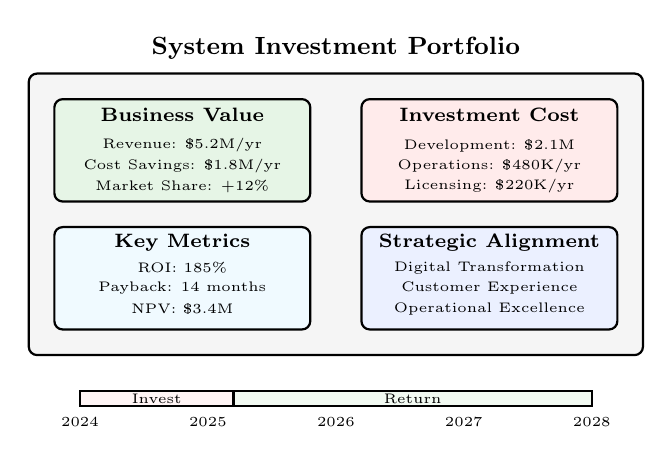
\begin{tikzpicture}[scale=0.65]
        % Value/Cost balance
        \draw[thick, fill=lightgray, rounded corners=3pt] (-6, 2) rectangle (6, -3.5);
        \node[font=\small\bfseries] at (0, 2.5) {System Investment Portfolio};
        
        % Value side
        \draw[thick, fill=valuecolor, rounded corners=3pt] (-5.5, 1.5) rectangle (-0.5, -0.5);
        \node[font=\scriptsize\bfseries] at (-3, 1.2) {Business Value};
        \node[font=\tiny] at (-3, 0.6) {Revenue: \$5.2M/yr};
        \node[font=\tiny] at (-3, 0.2) {Cost Savings: \$1.8M/yr};
        \node[font=\tiny] at (-3, -0.2) {Market Share: +12\%};
        
        % Cost side
        \draw[thick, fill=costcolor, rounded corners=3pt] (0.5, 1.5) rectangle (5.5, -0.5);
        \node[font=\scriptsize\bfseries] at (3, 1.2) {Investment Cost};
        \node[font=\tiny] at (3, 0.6) {Development: \$2.1M};
        \node[font=\tiny] at (3, 0.2) {Operations: \$480K/yr};
        \node[font=\tiny] at (3, -0.2) {Licensing: \$220K/yr};
        
        % KPIs
        \draw[thick, fill=kpicolor, rounded corners=3pt] (-5.5, -1) rectangle (-0.5, -3);
        \node[font=\scriptsize\bfseries] at (-3, -1.3) {Key Metrics};
        \node[font=\tiny] at (-3, -1.8) {ROI: 185\%};
        \node[font=\tiny] at (-3, -2.2) {Payback: 14 months};
        \node[font=\tiny] at (-3, -2.6) {NPV: \$3.4M};
        
        % Strategic alignment
        \draw[thick, fill=strategycolor, rounded corners=3pt] (0.5, -1) rectangle (5.5, -3);
        \node[font=\scriptsize\bfseries] at (3, -1.3) {Strategic Alignment};
        \node[font=\tiny] at (3, -1.8) {Digital Transformation};
        \node[font=\tiny] at (3, -2.2) {Customer Experience};
        \node[font=\tiny] at (3, -2.6) {Operational Excellence};
        
        % Timeline
        \draw[thick, darkgray] (-5, -4.5) -- (5, -4.5);
        \node[font=\tiny] at (-5, -4.8) {2024};
        \node[font=\tiny] at (-2.5, -4.8) {2025};
        \node[font=\tiny] at (0, -4.8) {2026};
        \node[font=\tiny] at (2.5, -4.8) {2027};
        \node[font=\tiny] at (5, -4.8) {2028};
        
        % Investment phases
        \draw[thick, fill=costcolor!50] (-5, -4.2) rectangle (-2, -4.5);
        \draw[thick, fill=valuecolor!50] (-2, -4.2) rectangle (5, -4.5);
        \node[font=\tiny] at (-3.5, -4.35) {Invest};
        \node[font=\tiny] at (1.5, -4.35) {Return};
        
    \end{tikzpicture}
    
    \vspace{1.3cm}
    
    \begin{tabular}{ll}
        \textbf{Version:} & 2.0 \\
        \textbf{Status:} & Release \\
        \textbf{Classification:} & ISO/IEC/IEEE 42010 Compliant \\
        \textbf{Last Updated:} & \today \\
    \end{tabular}
    
    \vfill
    
    {\small Based on the Views and Beyond approach to software architecture documentation}
    
\end{titlepage}
\hypersetup{pageanchor=true}

% -----------------------------------------------------------------------------
% TABLE OF CONTENTS
% -----------------------------------------------------------------------------
\tableofcontents
\newpage

% =============================================================================
% SECTION: VIEWPOINT NAME
% =============================================================================
\section{Viewpoint Name}

\begin{definitionbox}[Viewpoint Identification]
\begin{tabular}{@{}L{3.5cm}L{10cm}@{}}
\textbf{Name:} & Owner's View \\[0.5em]
\textbf{Synonyms:} & Business View, Executive View, Investment View, Sponsor's View, Economic View, Value View, Portfolio View \\[0.5em]
\textbf{Identifier:} & VP-OWN-001 \\[0.5em]
\textbf{Version:} & 2.0 \\
\end{tabular}
\end{definitionbox}

\subsection{Viewpoint Classification}

The Owner's View addresses the concerns of system owners, sponsors, and business executives. While not a traditional technical viewpoint in the Views and Beyond approach, it provides essential business context that guides architectural decisions. This viewpoint bridges business strategy and technical architecture, ensuring systems deliver value aligned with organizational goals.

\begin{table}[H]
\centering
\caption{Viewpoint Classification Taxonomy}
\begin{tabular}{@{}L{4cm}L{10cm}@{}}
\toprule
\textbf{Attribute} & \textbf{Value} \\
\midrule
Style Family & Business/Economic (Cross-cutting) \\
Primary Focus & Business Value, Cost, Strategy, Governance \\
Abstraction Level & Executive / Strategic \\
Temporal Perspective & Investment Lifecycle \\
Related Concepts & Business Case, ROI Analysis, Portfolio Management \\
IEEE 42010 Category & Stakeholder Concern Documentation \\
TOGAF Alignment & Business Architecture, Architecture Governance \\
\bottomrule
\end{tabular}
\end{table}

\subsection{Viewpoint Scope}

The Owner's View encompasses the following aspects:

\begin{itemize}
    \item \textbf{Business Value:} Quantified benefits the system delivers to the organization.
    
    \item \textbf{Investment and Cost:} Total cost of ownership including development and operations.
    
    \item \textbf{Strategic Alignment:} How the system supports business strategy and goals.
    
    \item \textbf{Risk Exposure:} Business and technical risks with financial implications.
    
    \item \textbf{Governance:} Decision rights, policies, and compliance requirements.
    
    \item \textbf{Lifecycle Economics:} Financial projections over the system's lifespan.
    
    \item \textbf{Portfolio Context:} Relationship to other systems and investments.
    
    \item \textbf{Success Metrics:} Key performance indicators measuring business outcomes.
\end{itemize}

% =============================================================================
% SECTION: OVERVIEW
% =============================================================================
\section{Overview}

The Owner's View provides business executives and sponsors with the information needed to make investment decisions, govern system development, and measure success. It translates technical architecture into business terms that stakeholders can evaluate against organizational priorities.

\subsection{Purpose and Scope}

The primary purpose of this viewpoint is to articulate the business justification for the system, track value delivery, and ensure alignment with strategic objectives. It enables informed decision-making about system investments, priorities, and trade-offs.

\begin{definitionbox}[Viewpoint Definition]
The Owner's View documents the business context, value proposition, investment requirements, strategic alignment, governance structure, and success metrics for a system. It provides executives and sponsors with the information needed to authorize, fund, govern, and evaluate system investments from a business perspective, ensuring technology decisions support organizational goals.
\end{definitionbox}

\subsection{Key Characteristics}

The Owner's View exhibits several distinctive characteristics:

\textbf{Business Language:} Uses business terminology rather than technical jargon, accessible to non-technical stakeholders.

\textbf{Quantified Value:} Expresses benefits and costs in financial and measurable terms.

\textbf{Strategic Focus:} Connects system capabilities to business strategy and competitive positioning.

\textbf{Decision Support:} Provides information for investment decisions, trade-offs, and prioritization.

\textbf{Accountability:} Establishes clear ownership, governance, and success criteria.

\subsection{Relationship to Other Viewpoints}

The Owner's View connects to other architectural viewpoints:

\begin{table}[H]
\centering
\caption{Relationships to Other Viewpoints}
\begin{tabular}{@{}L{3.5cm}L{10.5cm}@{}}
\toprule
\textbf{Viewpoint} & \textbf{Relationship} \\
\midrule
Logical/Functional & Business capabilities map to functional architecture. Value streams align with services. \\
\addlinespace
Context & External integrations have business relationships. Ecosystem partners provide/consume value. \\
\addlinespace
Deployment & Infrastructure costs contribute to TCO. Cloud vs on-premise affects financial model. \\
\addlinespace
Operational & Operations costs are part of TCO. SLAs tie to business commitments. \\
\addlinespace
Planner's & Development costs and timeline affect business case. Resource investment tracked. \\
\addlinespace
Security & Compliance requirements have cost/risk implications. Security incidents have business impact. \\
\bottomrule
\end{tabular}
\end{table}

\subsection{Business Architecture Overview}

\begin{figure}[H]
\centering
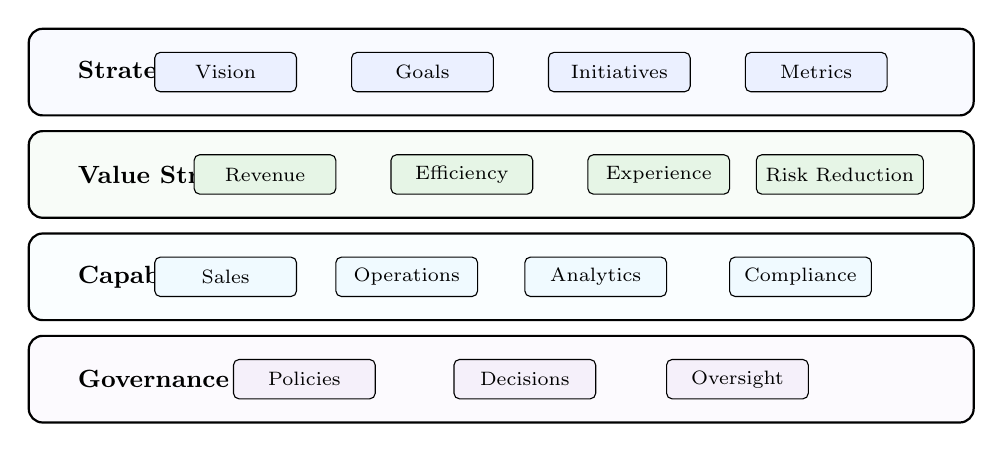
\begin{tikzpicture}[
    node distance=1cm and 1.5cm,
    layer/.style={draw, thick, rounded corners=5pt, minimum width=12cm, minimum height=1.1cm, font=\small},
    element/.style={draw, rounded corners=2pt, minimum width=1.8cm, minimum height=0.5cm, font=\scriptsize},
]
    % Layers
    \node[layer, fill=strategycolor!30] (strategy) at (0, 3.5) {};
    \node[font=\small\bfseries, anchor=west] at (-5.5, 3.5) {Strategy};
    
    \node[layer, fill=valuecolor!30] (value) at (0, 2.2) {};
    \node[font=\small\bfseries, anchor=west] at (-5.5, 2.2) {Value Streams};
    
    \node[layer, fill=kpicolor!30] (capability) at (0, 0.9) {};
    \node[font=\small\bfseries, anchor=west] at (-5.5, 0.9) {Capabilities};
    
    \node[layer, fill=governcolor!30] (governance) at (0, -0.4) {};
    \node[font=\small\bfseries, anchor=west] at (-5.5, -0.4) {Governance};
    
    % Strategy elements
    \node[element, fill=strategycolor] at (-3.5, 3.5) {Vision};
    \node[element, fill=strategycolor] at (-1, 3.5) {Goals};
    \node[element, fill=strategycolor] at (1.5, 3.5) {Initiatives};
    \node[element, fill=strategycolor] at (4, 3.5) {Metrics};
    
    % Value elements
    \node[element, fill=valuecolor] at (-3, 2.2) {Revenue};
    \node[element, fill=valuecolor] at (-0.5, 2.2) {Efficiency};
    \node[element, fill=valuecolor] at (2, 2.2) {Experience};
    \node[element, fill=valuecolor] at (4.3, 2.2) {Risk Reduction};
    
    % Capability elements
    \node[element, fill=kpicolor] at (-3.5, 0.9) {Sales};
    \node[element, fill=kpicolor] at (-1.2, 0.9) {Operations};
    \node[element, fill=kpicolor] at (1.2, 0.9) {Analytics};
    \node[element, fill=kpicolor] at (3.8, 0.9) {Compliance};
    
    % Governance elements
    \node[element, fill=governcolor] at (-2.5, -0.4) {Policies};
    \node[element, fill=governcolor] at (0.3, -0.4) {Decisions};
    \node[element, fill=governcolor] at (3, -0.4) {Oversight};
    
\end{tikzpicture}
\caption{Business Architecture Layers}
\end{figure}

% =============================================================================
% SECTION: CONCERNS
% =============================================================================
\section{Concerns}

This section enumerates the business concerns that the Owner's View is designed to address.

\subsection{Primary Concerns}

\begin{enumerate}[label=\textbf{C\arabic*:}, leftmargin=2.5em]
    \item \textbf{Business Value Delivery}
    \begin{itemize}[nosep]
        \item What business value does the system deliver?
        \item How is value quantified and measured?
        \item What revenue/savings does it generate?
        \item What competitive advantage does it provide?
        \item How does value accrue over time?
    \end{itemize}
    
    \item \textbf{Total Cost of Ownership}
    \begin{itemize}[nosep]
        \item What is the total investment required?
        \item What are development costs?
        \item What are ongoing operational costs?
        \item What are licensing and infrastructure costs?
        \item How do costs change over time?
    \end{itemize}
    
    \item \textbf{Return on Investment}
    \begin{itemize}[nosep]
        \item What is the expected ROI?
        \item What is the payback period?
        \item What is the net present value (NPV)?
        \item How does this compare to alternatives?
        \item What assumptions underlie projections?
    \end{itemize}
    
    \item \textbf{Strategic Alignment}
    \begin{itemize}[nosep]
        \item How does the system support business strategy?
        \item Which strategic initiatives does it enable?
        \item How does it affect competitive positioning?
        \item What business capabilities does it provide?
        \item How does it align with digital transformation?
    \end{itemize}
    
    \item \textbf{Risk Exposure}
    \begin{itemize}[nosep]
        \item What business risks does the system create/mitigate?
        \item What is the financial exposure from risks?
        \item What compliance/regulatory risks exist?
        \item What are the risks of not investing?
        \item How are risks monitored and managed?
    \end{itemize}
    
    \item \textbf{Governance and Control}
    \begin{itemize}[nosep]
        \item Who owns and sponsors the system?
        \item What decision rights exist?
        \item What policies govern the system?
        \item How is compliance ensured?
        \item What oversight mechanisms exist?
    \end{itemize}
    
    \item \textbf{Portfolio Context}
    \begin{itemize}[nosep]
        \item How does this system fit in the portfolio?
        \item What dependencies exist on other systems?
        \item What synergies or conflicts exist?
        \item How does it affect technical debt?
        \item What consolidation opportunities exist?
    \end{itemize}
    
    \item \textbf{Lifecycle Management}
    \begin{itemize}[nosep]
        \item What is the expected system lifespan?
        \item When will major upgrades be needed?
        \item What is the evolution roadmap?
        \item When should the system be retired?
        \item How is end-of-life managed?
    \end{itemize}
    
    \item \textbf{Success Metrics}
    \begin{itemize}[nosep]
        \item How is success defined?
        \item What KPIs track business outcomes?
        \item How are metrics collected and reported?
        \item What targets are set?
        \item How are deviations addressed?
    \end{itemize}
    
    \item \textbf{Stakeholder Impact}
    \begin{itemize}[nosep]
        \item Who are the business stakeholders?
        \item How does the system affect customers?
        \item What is the employee impact?
        \item How are partners affected?
        \item What change management is needed?
    \end{itemize}
\end{enumerate}

\subsection{Concern-Business Outcome Mapping}

\begin{table}[H]
\centering
\caption{Concern to Business Outcome Mapping}
\small
\begin{tabular}{@{}L{2.8cm}C{1cm}C{1cm}C{1cm}C{1cm}C{1cm}C{1cm}C{1cm}C{1cm}@{}}
\toprule
\textbf{Concern} & \rotatebox{60}{\textbf{Revenue}} & \rotatebox{60}{\textbf{Cost Red.}} & \rotatebox{60}{\textbf{Efficiency}} & \rotatebox{60}{\textbf{Cust. Exp.}} & \rotatebox{60}{\textbf{Compliance}} & \rotatebox{60}{\textbf{Agility}} & \rotatebox{60}{\textbf{Risk Red.}} & \rotatebox{60}{\textbf{Innovation}} \\
\midrule
Value Delivery & $\bullet$ & $\bullet$ & $\bullet$ & $\bullet$ & $\circ$ & $\circ$ & $\circ$ & $\circ$ \\
Total Cost & $\circ$ & $\bullet$ & $\bullet$ & -- & -- & $\circ$ & $\circ$ & -- \\
ROI & $\bullet$ & $\bullet$ & $\circ$ & $\circ$ & -- & -- & -- & -- \\
Strategy & $\bullet$ & $\circ$ & $\circ$ & $\bullet$ & $\circ$ & $\bullet$ & $\circ$ & $\bullet$ \\
Risk Exposure & $\circ$ & $\circ$ & -- & $\circ$ & $\bullet$ & -- & $\bullet$ & -- \\
Governance & -- & $\circ$ & $\circ$ & -- & $\bullet$ & $\circ$ & $\bullet$ & -- \\
Portfolio & $\circ$ & $\bullet$ & $\bullet$ & $\circ$ & $\circ$ & $\bullet$ & $\circ$ & $\circ$ \\
Lifecycle & $\circ$ & $\bullet$ & $\circ$ & -- & $\circ$ & $\bullet$ & $\circ$ & $\bullet$ \\
Success Metrics & $\bullet$ & $\bullet$ & $\bullet$ & $\bullet$ & $\bullet$ & $\circ$ & $\circ$ & $\circ$ \\
Stakeholder & $\bullet$ & $\circ$ & $\circ$ & $\bullet$ & $\circ$ & $\circ$ & $\circ$ & $\circ$ \\
\bottomrule
\multicolumn{9}{l}{\footnotesize $\bullet$ = Primary impact, $\circ$ = Secondary impact, -- = Minimal impact}
\end{tabular}
\end{table}

% =============================================================================
% SECTION: ANTI-CONCERNS
% =============================================================================
\section{Anti-Concerns}

Understanding what the Owner's View is \emph{not} appropriate for helps stakeholders avoid misapplying this viewpoint.

\subsection{Out of Scope Topics}

\begin{enumerate}[label=\textbf{AC\arabic*:}, leftmargin=2.5em]
    \item \textbf{Technical Implementation Details}
    \begin{itemize}[nosep]
        \item Programming languages and frameworks
        \item Database design and schemas
        \item API specifications
        \item Algorithm implementations
        \item Code structure and patterns
    \end{itemize}
    
    \item \textbf{Detailed System Design}
    \begin{itemize}[nosep]
        \item Component interactions
        \item Data flow details
        \item Interface specifications
        \item Concurrency design
        \item Error handling approaches
    \end{itemize}
    
    \item \textbf{Operational Procedures}
    \begin{itemize}[nosep]
        \item Deployment scripts
        \item Monitoring configuration
        \item Incident runbooks
        \item Backup procedures
        \item Performance tuning
    \end{itemize}
    
    \item \textbf{Development Process Details}
    \begin{itemize}[nosep]
        \item Sprint planning
        \item Code review processes
        \item Testing strategies
        \item CI/CD pipeline details
        \item Developer workflows
    \end{itemize}
    
    \item \textbf{Detailed Project Management}
    \begin{itemize}[nosep]
        \item Task-level scheduling
        \item Resource allocation details
        \item Individual assignments
        \item Daily status tracking
        \item Bug tracking
    \end{itemize}
\end{enumerate}

\begin{warningbox}[Common Misapplications]
Avoid using the Owner's View for:

\begin{itemize}[nosep]
    \item Making technical design decisions (use technical viewpoints)
    \item Detailed project planning (use Planner's View)
    \item Operational procedures (use Operational Viewpoint)
    \item Development guidance (use Development Viewpoint)
    \item Detailed requirements (use Requirements documents)
\end{itemize}
\end{warningbox}

% =============================================================================
% SECTION: TYPICAL STAKEHOLDERS
% =============================================================================
\section{Typical Stakeholders}

The Owner's View serves stakeholders involved in business decisions and governance.

\subsection{Primary Stakeholders}

\begin{table}[H]
\centering
\caption{Primary Stakeholder Analysis}
\small
\begin{tabular}{@{}L{2.6cm}L{3.6cm}L{7cm}@{}}
\toprule
\textbf{Stakeholder} & \textbf{Role Description} & \textbf{Primary Interests} \\
\midrule
Executive Sponsor & Authorizes and funds system & ROI, strategic alignment, risk, business outcomes \\
\addlinespace
Business Owner & Accountable for value delivery & Value realization, KPIs, capability delivery \\
\addlinespace
CFO/Finance & Controls investment budget & TCO, ROI, cash flow, financial projections \\
\addlinespace
CIO/CTO & Technology strategy leader & Portfolio fit, technical debt, strategic alignment \\
\addlinespace
Product Owner & Defines business requirements & Feature value, customer impact, prioritization \\
\addlinespace
Board/Investors & Governance and oversight & Strategic value, risk exposure, compliance \\
\bottomrule
\end{tabular}
\end{table}

\subsection{Secondary Stakeholders}

\begin{table}[H]
\centering
\caption{Secondary Stakeholder Analysis}
\small
\begin{tabular}{@{}L{2.6cm}L{3.6cm}L{7cm}@{}}
\toprule
\textbf{Stakeholder} & \textbf{Role Description} & \textbf{Primary Interests} \\
\midrule
Enterprise Architect & Manages architecture portfolio & Strategic alignment, standards, integration \\
\addlinespace
Program Manager & Coordinates delivery programs & Timeline, dependencies, resource needs \\
\addlinespace
Compliance Officer & Ensures regulatory compliance & Regulatory requirements, audit, risk \\
\addlinespace
Legal Counsel & Manages legal obligations & Contracts, liability, IP, privacy \\
\addlinespace
Business Analysts & Define business requirements & Business processes, requirements traceability \\
\addlinespace
Change Manager & Manages organizational change & Stakeholder impact, adoption, training \\
\bottomrule
\end{tabular}
\end{table}

\subsection{Stakeholder Concern Matrix}

\begin{table}[H]
\centering
\caption{Stakeholder-Concern Responsibility Matrix}
\footnotesize
\begin{tabular}{@{}L{2cm}C{0.8cm}C{0.8cm}C{0.8cm}C{0.8cm}C{0.8cm}C{0.8cm}C{0.8cm}C{0.8cm}C{0.8cm}C{0.8cm}@{}}
\toprule
& \rotatebox{60}{\textbf{Value}} & \rotatebox{60}{\textbf{Cost}} & \rotatebox{60}{\textbf{ROI}} & \rotatebox{60}{\textbf{Strategy}} & \rotatebox{60}{\textbf{Risk}} & \rotatebox{60}{\textbf{Govern.}} & \rotatebox{60}{\textbf{Portfolio}} & \rotatebox{60}{\textbf{Lifecycle}} & \rotatebox{60}{\textbf{Metrics}} & \rotatebox{60}{\textbf{Stakehld}} \\
\midrule
Sponsor & A & A & A & R & A & R & C & C & A & R \\
Bus. Owner & R & C & C & C & R & C & I & R & R & R \\
CFO & C & R & R & C & R & C & R & C & C & I \\
CIO/CTO & C & C & C & R & R & R & R & R & C & C \\
Prod. Owner & R & I & I & C & C & I & I & C & R & R \\
Board & I & I & A & A & A & A & I & I & I & I \\
\bottomrule
\multicolumn{11}{l}{\footnotesize R = Responsible, A = Accountable, C = Consulted, I = Informed}
\end{tabular}
\end{table}

% =============================================================================
% SECTION: MODEL TYPES
% =============================================================================
\section{Model Types}

The Owner's View employs several complementary model types to capture different aspects of business context and value.

\subsection{Model Type Catalog}

\begin{enumerate}[label=\textbf{MT\arabic*:}, leftmargin=2.5em]
    \item \textbf{Business Case Summary}
    \begin{itemize}[nosep]
        \item \textit{Purpose:} Document investment justification
        \item \textit{Primary Elements:} Value proposition, costs, benefits, ROI
        \item \textit{Key Relationships:} Investment yields returns
        \item \textit{Typical Notation:} Executive summary, financial tables
    \end{itemize}
    
    \item \textbf{Value Stream Map}
    \begin{itemize}[nosep]
        \item \textit{Purpose:} Show how value flows to customers
        \item \textit{Primary Elements:} Value activities, handoffs, metrics
        \item \textit{Key Relationships:} Enables, flows-to
        \item \textit{Typical Notation:} Value stream diagrams
    \end{itemize}
    
    \item \textbf{Strategic Alignment Matrix}
    \begin{itemize}[nosep]
        \item \textit{Purpose:} Map system to strategic objectives
        \item \textit{Primary Elements:} Goals, initiatives, capabilities
        \item \textit{Key Relationships:} Supports, enables, contributes-to
        \item \textit{Typical Notation:} Alignment matrices, strategy maps
    \end{itemize}
    
    \item \textbf{Total Cost of Ownership Model}
    \begin{itemize}[nosep]
        \item \textit{Purpose:} Detail all costs over system lifecycle
        \item \textit{Primary Elements:} Cost categories, time periods
        \item \textit{Key Relationships:} Comprises, varies-with
        \item \textit{Typical Notation:} Cost breakdown tables, projections
    \end{itemize}
    
    \item \textbf{Financial Projection Model}
    \begin{itemize}[nosep]
        \item \textit{Purpose:} Project financial outcomes
        \item \textit{Primary Elements:} Cash flows, ROI, NPV, IRR
        \item \textit{Key Relationships:} Generates, requires
        \item \textit{Typical Notation:} Financial statements, charts
    \end{itemize}
    
    \item \textbf{Risk Register (Business)}
    \begin{itemize}[nosep]
        \item \textit{Purpose:} Document business risks and impacts
        \item \textit{Primary Elements:} Risks, impacts, mitigations
        \item \textit{Key Relationships:} Affects, mitigates
        \item \textit{Typical Notation:} Risk tables, heat maps
    \end{itemize}
    
    \item \textbf{Governance Framework}
    \begin{itemize}[nosep]
        \item \textit{Purpose:} Define decision rights and oversight
        \item \textit{Primary Elements:} Roles, decisions, processes
        \item \textit{Key Relationships:} Authorizes, oversees, approves
        \item \textit{Typical Notation:} RACI matrices, governance charts
    \end{itemize}
    
    \item \textbf{KPI Dashboard}
    \begin{itemize}[nosep]
        \item \textit{Purpose:} Track business success metrics
        \item \textit{Primary Elements:} Metrics, targets, actuals
        \item \textit{Key Relationships:} Measures, indicates
        \item \textit{Typical Notation:} Dashboards, scorecards
    \end{itemize}
    
    \item \textbf{Portfolio View}
    \begin{itemize}[nosep]
        \item \textit{Purpose:} Show system in portfolio context
        \item \textit{Primary Elements:} Systems, relationships, investments
        \item \textit{Key Relationships:} Integrates-with, replaces, depends-on
        \item \textit{Typical Notation:} Portfolio maps, bubble charts
    \end{itemize}
\end{enumerate}

\subsection{Model Type Relationships}

\begin{figure}[H]
\centering
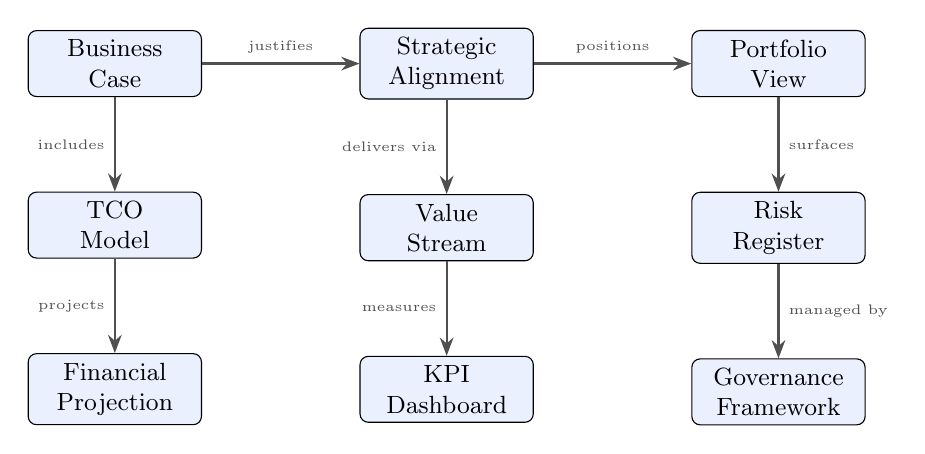
\begin{tikzpicture}[
    node distance=1.2cm and 2cm,
    model/.style={draw, fill=strategycolor, rounded corners=3pt, minimum width=2.2cm, minimum height=0.7cm, font=\small, align=center},
    arrow/.style={-{Stealth}, thick, darkgray}
]
    % Nodes - top row
    \node[model] (bizcase) {Business\\Case};
    \node[model, right=2cm of bizcase] (strategy) {Strategic\\Alignment};
    \node[model, right=2cm of strategy] (portfolio) {Portfolio\\View};
    
    % Nodes - middle row
    \node[model, below=1.2cm of bizcase] (tco) {TCO\\Model};
    \node[model, below=1.2cm of strategy] (value) {Value\\Stream};
    \node[model, below=1.2cm of portfolio] (risk) {Risk\\Register};
    
    % Nodes - bottom row
    \node[model, below=1.2cm of tco] (financial) {Financial\\Projection};
    \node[model, below=1.2cm of value] (kpi) {KPI\\Dashboard};
    \node[model, below=1.2cm of risk] (govern) {Governance\\Framework};
    
    % Arrows
    \draw[arrow] (bizcase) -- (strategy) node[midway, above, font=\tiny] {justifies};
    \draw[arrow] (strategy) -- (portfolio) node[midway, above, font=\tiny] {positions};
    \draw[arrow] (bizcase) -- (tco) node[midway, left, font=\tiny] {includes};
    \draw[arrow] (tco) -- (financial) node[midway, left, font=\tiny] {projects};
    \draw[arrow] (strategy) -- (value) node[midway, left, font=\tiny] {delivers via};
    \draw[arrow] (value) -- (kpi) node[midway, left, font=\tiny] {measures};
    \draw[arrow] (portfolio) -- (risk) node[midway, right, font=\tiny] {surfaces};
    \draw[arrow] (risk) -- (govern) node[midway, right, font=\tiny] {managed by};
\end{tikzpicture}
\caption{Model Type Dependency Relationships}
\end{figure}

% =============================================================================
% SECTION: MODEL LANGUAGES
% =============================================================================
\section{Model Languages}

For each model type, specific languages, notations, and techniques are prescribed.

\subsection{Business Value Notation}

\begin{figure}[H]
\centering
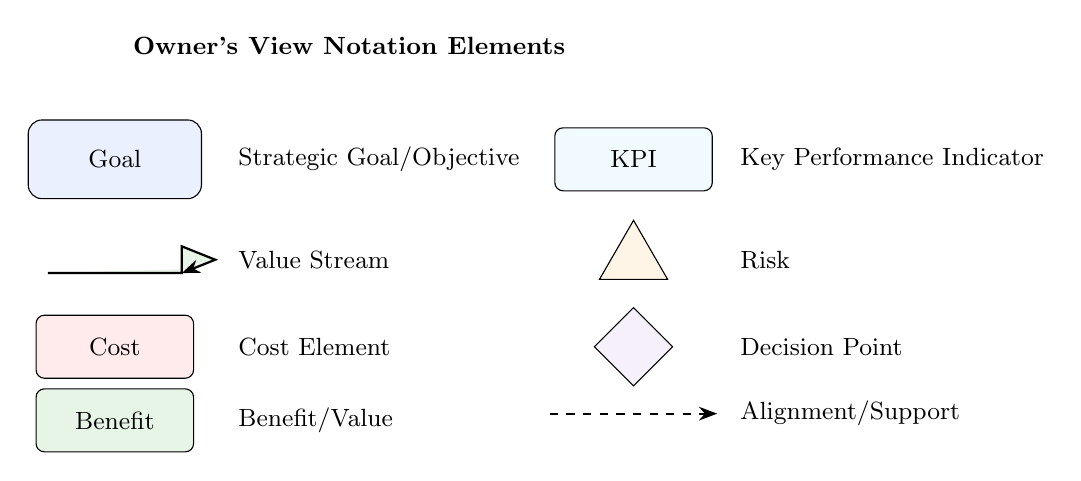
\begin{tikzpicture}[scale=0.85]
    % Legend title
    \node[font=\small\bfseries] at (0, 5) {Owner's View Notation Elements};
    
    % Strategic goal
    \node[draw, fill=strategycolor, rounded corners=5pt, minimum width=2.2cm, minimum height=1cm] at (-3.5, 3.3) {};
    \node[font=\small] at (-3.5, 3.3) {Goal};
    \node[right, font=\small] at (-1.8, 3.3) {Strategic Goal/Objective};
    
    % Value stream
    \draw[thick, fill=valuecolor, -{Stealth}] (-4.5, 1.6) -- (-2.5, 1.6) -- (-2.5, 2) -- (-2, 1.8) -- (-2.5, 1.6);
    \node[right, font=\small] at (-1.8, 1.8) {Value Stream};
    
    % Cost
    \node[draw, fill=costcolor, rounded corners=3pt, minimum width=2cm, minimum height=0.8cm] at (-3.5, 0.5) {};
    \node[font=\small] at (-3.5, 0.5) {Cost};
    \node[right, font=\small] at (-1.8, 0.5) {Cost Element};
    
    % Benefit
    \node[draw, fill=valuecolor, rounded corners=3pt, minimum width=2cm, minimum height=0.8cm] at (-3.5, -0.6) {};
    \node[font=\small] at (-3.5, -0.6) {Benefit};
    \node[right, font=\small] at (-1.8, -0.6) {Benefit/Value};
    
    % KPI
    \node[draw, fill=kpicolor, rounded corners=3pt, minimum width=2cm, minimum height=0.8cm] at (4.25, 3.3) {};
    \node[font=\small] at (4.25, 3.3) {KPI};
    \node[right, font=\small] at (5.7, 3.3) {Key Performance Indicator};
    
    % Risk
    \node[draw, fill=riskcolor, regular polygon, regular polygon sides=3, minimum size=1cm] at (4.25, 1.8) {};
    \node[right, font=\small] at (5.7, 1.8) {Risk};
    
    % Decision
    \node[draw, fill=governcolor, diamond, minimum size=1cm] at (4.25, 0.5) {};
    \node[right, font=\small] at (5.7, 0.5) {Decision Point};
    
    % Alignment arrow
    \draw[-{Stealth}, thick, dashed] (3, -0.5) -- (5.5, -0.5);
    \node[right, font=\small] at (5.7, -0.5) {Alignment/Support};
    
\end{tikzpicture}
\caption{Owner's View Notation Legend}
\end{figure}

\subsection{Value Type Classifications}

\begin{table}[H]
\centering
\caption{Business Value Type Classification}
\small
\begin{tabular}{@{}L{2.5cm}L{4.5cm}L{5.5cm}@{}}
\toprule
\textbf{Value Type} & \textbf{Description} & \textbf{Examples} \\
\midrule
Revenue Generation & Direct contribution to income & New sales channels, upsell, market expansion \\
\addlinespace
Cost Reduction & Decrease in operating expenses & Automation, efficiency, consolidation \\
\addlinespace
Cost Avoidance & Prevention of future costs & Risk mitigation, compliance, prevention \\
\addlinespace
Productivity & Improved output per resource & Process automation, better tools \\
\addlinespace
Customer Value & Improved customer outcomes & Experience, satisfaction, retention \\
\addlinespace
Strategic Value & Competitive or market positioning & Market share, brand, differentiation \\
\addlinespace
Risk Reduction & Decreased risk exposure & Security, compliance, resilience \\
\addlinespace
Enablement & Foundation for future value & Platform, capabilities, data \\
\bottomrule
\end{tabular}
\end{table}

\subsection{Cost Type Classifications}

\begin{table}[H]
\centering
\caption{Cost Type Classification}
\small
\begin{tabular}{@{}L{2.5cm}L{4cm}L{6cm}@{}}
\toprule
\textbf{Cost Type} & \textbf{Description} & \textbf{Components} \\
\midrule
Development & Building the system & Labor, contractors, tools, training \\
\addlinespace
Infrastructure & Hosting and compute & Cloud services, hardware, network, storage \\
\addlinespace
Licensing & Software licenses & Commercial software, SaaS subscriptions \\
\addlinespace
Operations & Running the system & Support staff, monitoring, maintenance \\
\addlinespace
Integration & Connecting systems & APIs, middleware, data migration \\
\addlinespace
Change Management & Organizational change & Training, communications, adoption \\
\addlinespace
Compliance & Meeting regulations & Audits, certifications, controls \\
\addlinespace
Opportunity & Alternative use of funds & Foregone investments, delayed projects \\
\bottomrule
\end{tabular}
\end{table}

\subsection{Financial Metrics}

\begin{table}[H]
\centering
\caption{Key Financial Metrics}
\small
\begin{tabular}{@{}L{2.5cm}L{5cm}L{5cm}@{}}
\toprule
\textbf{Metric} & \textbf{Definition} & \textbf{Formula/Calculation} \\
\midrule
ROI & Return on Investment & $(Benefits - Costs) / Costs \times 100\%$ \\
\addlinespace
NPV & Net Present Value & $\sum_{t=0}^{n} \frac{CF_t}{(1+r)^t}$ \\
\addlinespace
IRR & Internal Rate of Return & Rate where $NPV = 0$ \\
\addlinespace
Payback Period & Time to recover investment & Time when cumulative CF $> 0$ \\
\addlinespace
TCO & Total Cost of Ownership & All costs over system lifetime \\
\addlinespace
EVA & Economic Value Added & $NOPAT - (Capital \times WACC)$ \\
\bottomrule
\end{tabular}
\end{table}

\subsection{Tabular Specifications}

\subsubsection{Business Case Summary Table}

\begin{table}[H]
\centering
\caption{Example Business Case Summary}
\small
\begin{tabular}{@{}L{4cm}R{3cm}L{5.5cm}@{}}
\toprule
\textbf{Item} & \textbf{Value} & \textbf{Notes} \\
\midrule
\multicolumn{3}{l}{\textbf{Investment Required}} \\
\quad Development Cost & \$2,100,000 & 18-month development \\
\quad Infrastructure Setup & \$180,000 & Cloud infrastructure \\
\quad Change Management & \$120,000 & Training, adoption \\
\quad \textbf{Total Investment} & \textbf{\$2,400,000} & \\
\midrule
\multicolumn{3}{l}{\textbf{Annual Benefits (Year 2+)}} \\
\quad Revenue Increase & \$3,200,000 & New channel, upsell \\
\quad Cost Savings & \$1,800,000 & Automation, efficiency \\
\quad \textbf{Total Annual Benefit} & \textbf{\$5,000,000} & \\
\midrule
\multicolumn{3}{l}{\textbf{Annual Costs (Year 2+)}} \\
\quad Operations & \$480,000 & Team, support \\
\quad Infrastructure & \$320,000 & Cloud costs \\
\quad Licensing & \$200,000 & Software licenses \\
\quad \textbf{Total Annual Cost} & \textbf{\$1,000,000} & \\
\midrule
\multicolumn{3}{l}{\textbf{Financial Metrics (5-year)}} \\
\quad Net Annual Benefit & \$4,000,000 & Benefits - Costs \\
\quad ROI & 185\% & \\
\quad Payback Period & 14 months & \\
\quad NPV (10\% discount) & \$8,400,000 & \\
\bottomrule
\end{tabular}
\end{table}

\subsubsection{Strategic Alignment Table}

\begin{table}[H]
\centering
\caption{Example Strategic Alignment Matrix}
\small
\begin{tabular}{@{}L{3.5cm}L{3cm}C{1.5cm}L{4cm}@{}}
\toprule
\textbf{Strategic Goal} & \textbf{System Capability} & \textbf{Impact} & \textbf{Contribution} \\
\midrule
Digital Transformation & Customer Portal & \cellcolor{green!30}High & Self-service, 24/7 access \\
\addlinespace
Customer Experience & Personalization & \cellcolor{green!30}High & Tailored recommendations \\
\addlinespace
Operational Excellence & Process Automation & \cellcolor{green!30}High & 60\% manual reduction \\
\addlinespace
Market Expansion & Multi-region Support & \cellcolor{yellow!30}Medium & Global deployment ready \\
\addlinespace
Data-Driven Decisions & Analytics Platform & \cellcolor{yellow!30}Medium & Real-time dashboards \\
\bottomrule
\end{tabular}
\end{table}

\subsubsection{KPI Definition Table}

\begin{table}[H]
\centering
\caption{Example KPI Definitions}
\small
\begin{tabular}{@{}L{2.5cm}L{3cm}C{1.5cm}C{1.5cm}L{3cm}@{}}
\toprule
\textbf{KPI} & \textbf{Definition} & \textbf{Target} & \textbf{Current} & \textbf{Data Source} \\
\midrule
Conversion Rate & Orders / Visitors & 4.5\% & 3.2\% & Analytics platform \\
\addlinespace
Avg Order Value & Revenue / Orders & \$125 & \$98 & Order system \\
\addlinespace
Customer Sat. & NPS Score & 50 & 42 & Survey system \\
\addlinespace
Processing Time & Order to ship (hrs) & 4 & 8 & Operations system \\
\addlinespace
System Uptime & Available time \% & 99.9\% & 99.5\% & Monitoring \\
\bottomrule
\end{tabular}
\end{table}

% =============================================================================
% SECTION: VIEWPOINT METAMODELS
% =============================================================================
\section{Viewpoint Metamodels}

This section defines the conceptual metamodel underlying the Owner's View.

\subsection{Core Metamodel}

\begin{figure}[H]
\centering
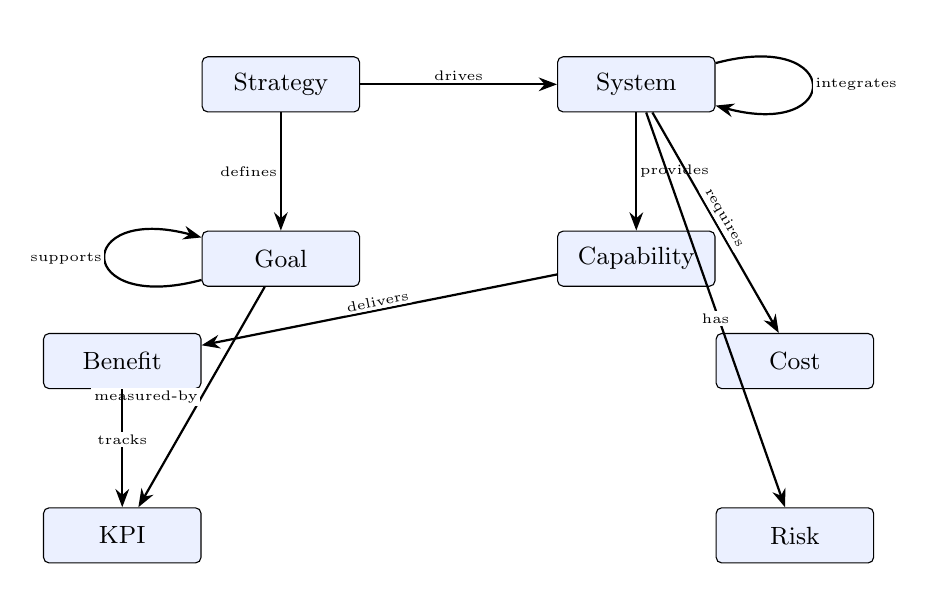
\begin{tikzpicture}[
    node distance=1.3cm and 2cm,
    entity/.style={draw, fill=strategycolor, rounded corners=2pt, minimum width=2cm, minimum height=0.7cm, font=\small},
    arrow/.style={-{Stealth}, thick},
    label/.style={font=\tiny, fill=white, inner sep=1pt}
]
    % Main entities
    \node[entity] (strategy) {Strategy};
    \node[entity, right=2.5cm of strategy] (system) {System};
    \node[entity, below=1.5cm of strategy] (goal) {Goal};
    \node[entity, below=1.5cm of system] (capability) {Capability};
    \node[entity, below left=2.8cm and 0cm of strategy] (benefit) {Benefit};
    \node[entity, below right=2.8cm and 0cm of system] (cost) {Cost};
    \node[entity, below=1.5cm of benefit] (kpi) {KPI};
    \node[entity, below=1.5cm of cost] (risk) {Risk};
    
    % Relationships
    \draw[arrow] (strategy) -- (system) node[label, midway, above] {drives};
    \draw[arrow] (strategy) -- (goal) node[label, midway, left] {defines};
    \draw[arrow] (system) -- (capability) node[label, midway, right] {provides};
    \draw[arrow] (capability) -- (benefit) node[label, midway, above, sloped] {delivers};
    \draw[arrow] (system) -- (cost) node[label, midway, above, sloped] {requires};
    \draw[arrow] (goal) -- (kpi) node[label, midway, left] {measured-by};
    \draw[arrow] (system) -- (risk) node[label, midway, below] {has};
    \draw[arrow] (benefit) -- (kpi) node[label, midway, above] {tracks};
    
    % Self-reference
    \draw[arrow] (goal) to[loop left] node[label, left] {supports} (goal);
    \draw[arrow] (system) to[loop right] node[label, right] {integrates} (system);
\end{tikzpicture}
\caption{Owner's View Core Metamodel}
\end{figure}

\subsection{Entity Definitions}

\begin{definitionbox}[Entity: Strategy]
\textbf{Definition:} The overarching business direction and priorities that guide system investments and decisions.

\textbf{Attributes:}
\begin{itemize}[nosep]
    \item \texttt{strategyId}: Unique identifier
    \item \texttt{name}: Strategy name
    \item \texttt{vision}: Long-term vision statement
    \item \texttt{mission}: Organization mission
    \item \texttt{timeHorizon}: Strategic planning period
    \item \texttt{themes}: Key strategic themes
    \item \texttt{priorities}: Ranked priorities
    \item \texttt{constraints}: Strategic constraints
    \item \texttt{owner}: Strategy owner (executive)
\end{itemize}

\textbf{Constraints:}
\begin{itemize}[nosep]
    \item Strategy should be documented and communicated
    \item Priorities should be ranked and clear
    \item Time horizon should be defined
\end{itemize}
\end{definitionbox}

\begin{definitionbox}[Entity: Goal]
\textbf{Definition:} A specific, measurable business objective that the system should help achieve.

\textbf{Attributes:}
\begin{itemize}[nosep]
    \item \texttt{goalId}: Unique identifier
    \item \texttt{name}: Goal name
    \item \texttt{description}: Goal description
    \item \texttt{type}: Goal type (financial, customer, operational, growth)
    \item \texttt{target}: Quantified target
    \item \texttt{timeframe}: Achievement timeframe
    \item \texttt{baseline}: Current state/baseline
    \item \texttt{owner}: Goal owner
    \item \texttt{parentGoal}: Parent goal if hierarchical
    \item \texttt{kpis}: Associated KPIs
\end{itemize}

\textbf{Constraints:}
\begin{itemize}[nosep]
    \item Goals should be SMART (Specific, Measurable, Achievable, Relevant, Time-bound)
    \item Goals should have clear ownership
    \item Progress should be measurable
\end{itemize}
\end{definitionbox}

\begin{definitionbox}[Entity: System]
\textbf{Definition:} The software system being evaluated from a business perspective, representing the investment.

\textbf{Attributes:}
\begin{itemize}[nosep]
    \item \texttt{systemId}: Unique identifier
    \item \texttt{name}: System name
    \item \texttt{description}: System purpose
    \item \texttt{sponsor}: Executive sponsor
    \item \texttt{owner}: Business owner
    \item \texttt{status}: Current status (planning, development, production, sunset)
    \item \texttt{lifecycleStage}: Stage in investment lifecycle
    \item \texttt{capabilities}: Provided business capabilities
    \item \texttt{portfolio}: Portfolio classification
    \item \texttt{criticality}: Business criticality rating
\end{itemize}

\textbf{Constraints:}
\begin{itemize}[nosep]
    \item System should have clear sponsorship and ownership
    \item Criticality should be assessed
    \item Portfolio position should be defined
\end{itemize}
\end{definitionbox}

\begin{definitionbox}[Entity: Capability]
\textbf{Definition:} A business ability that the system provides, contributing to business value.

\textbf{Attributes:}
\begin{itemize}[nosep]
    \item \texttt{capabilityId}: Unique identifier
    \item \texttt{name}: Capability name
    \item \texttt{description}: Capability description
    \item \texttt{type}: Capability type (core, supporting, enabling)
    \item \texttt{maturity}: Current maturity level
    \item \texttt{targetMaturity}: Target maturity
    \item \texttt{benefits}: Associated benefits
    \item \texttt{dependencies}: Dependent capabilities
    \item \texttt{owner}: Business owner
\end{itemize}

\textbf{Constraints:}
\begin{itemize}[nosep]
    \item Capabilities should map to business outcomes
    \item Maturity should be assessed
    \item Dependencies should be identified
\end{itemize}
\end{definitionbox}

\begin{definitionbox}[Entity: Benefit]
\textbf{Definition:} A positive business outcome or value delivered by the system.

\textbf{Attributes:}
\begin{itemize}[nosep]
    \item \texttt{benefitId}: Unique identifier
    \item \texttt{name}: Benefit name
    \item \texttt{description}: Benefit description
    \item \texttt{type}: Benefit type (revenue, cost reduction, productivity, etc.)
    \item \texttt{value}: Quantified value (monetary)
    \item \texttt{confidence}: Confidence level in estimate
    \item \texttt{timing}: When benefit is realized
    \item \texttt{recurringPeriod}: If recurring, the period
    \item \texttt{assumptions}: Key assumptions
    \item \texttt{owner}: Benefit owner
    \item \texttt{realization}: Realized vs projected
\end{itemize}

\textbf{Constraints:}
\begin{itemize}[nosep]
    \item Benefits should be quantified where possible
    \item Assumptions should be documented
    \item Realization should be tracked
\end{itemize}
\end{definitionbox}

\begin{definitionbox}[Entity: Cost]
\textbf{Definition:} An expenditure required to develop, operate, or maintain the system.

\textbf{Attributes:}
\begin{itemize}[nosep]
    \item \texttt{costId}: Unique identifier
    \item \texttt{name}: Cost name
    \item \texttt{description}: Cost description
    \item \texttt{type}: Cost type (development, operations, licensing, etc.)
    \item \texttt{category}: Capital vs operational
    \item \texttt{amount}: Cost amount
    \item \texttt{frequency}: One-time vs recurring
    \item \texttt{timing}: When cost is incurred
    \item \texttt{variability}: Fixed vs variable
    \item \texttt{confidence}: Confidence in estimate
    \item \texttt{actual}: Actual vs estimated
\end{itemize}

\textbf{Constraints:}
\begin{itemize}[nosep]
    \item Costs should be categorized appropriately
    \item Timing should be specified
    \item Actuals should be tracked against estimates
\end{itemize}
\end{definitionbox}

\begin{definitionbox}[Entity: KPI]
\textbf{Definition:} A Key Performance Indicator measuring business outcomes or system success.

\textbf{Attributes:}
\begin{itemize}[nosep]
    \item \texttt{kpiId}: Unique identifier
    \item \texttt{name}: KPI name
    \item \texttt{description}: KPI definition
    \item \texttt{formula}: Calculation method
    \item \texttt{target}: Target value
    \item \texttt{threshold}: Warning thresholds
    \item \texttt{frequency}: Measurement frequency
    \item \texttt{dataSource}: Source of data
    \item \texttt{owner}: KPI owner
    \item \texttt{current}: Current value
    \item \texttt{trend}: Trend direction
\end{itemize}

\textbf{Constraints:}
\begin{itemize}[nosep]
    \item KPIs should be measurable and actionable
    \item Targets should be realistic and time-bound
    \item Data sources should be reliable
\end{itemize}
\end{definitionbox}

\begin{definitionbox}[Entity: Risk (Business)]
\textbf{Definition:} A potential event or condition that could negatively impact business outcomes or investment returns.

\textbf{Attributes:}
\begin{itemize}[nosep]
    \item \texttt{riskId}: Unique identifier
    \item \texttt{name}: Risk name
    \item \texttt{description}: Risk description
    \item \texttt{category}: Risk category (market, operational, technical, regulatory)
    \item \texttt{probability}: Likelihood of occurrence
    \item \texttt{impact}: Financial/business impact
    \item \texttt{exposure}: Risk exposure (probability $\times$ impact)
    \item \texttt{mitigation}: Mitigation strategy
    \item \texttt{owner}: Risk owner
    \item \texttt{status}: Current status
    \item \texttt{trigger}: Early warning indicators
\end{itemize}

\textbf{Constraints:}
\begin{itemize}[nosep]
    \item High-exposure risks must have mitigation plans
    \item Business impact should be quantified
    \item Ownership should be assigned
\end{itemize}
\end{definitionbox}

\subsection{Relationship Definitions}

\begin{table}[H]
\centering
\caption{Metamodel Relationship Definitions}
\small
\begin{tabular}{@{}L{2.3cm}L{1.8cm}L{1.8cm}L{7.5cm}@{}}
\toprule
\textbf{Relationship} & \textbf{Source} & \textbf{Target} & \textbf{Description} \\
\midrule
drives & Strategy & System & Strategy directs system investment \\
\addlinespace
defines & Strategy & Goal & Strategy establishes goals \\
\addlinespace
provides & System & Capability & System delivers capability \\
\addlinespace
delivers & Capability & Benefit & Capability produces benefit \\
\addlinespace
requires & System & Cost & System incurs cost \\
\addlinespace
measured-by & Goal & KPI & Goal is tracked by KPI \\
\addlinespace
has & System & Risk & System carries risk \\
\addlinespace
tracks & Benefit & KPI & Benefit is measured by KPI \\
\addlinespace
supports & Goal & Goal & Goal contributes to parent goal \\
\addlinespace
integrates & System & System & Systems interact in portfolio \\
\bottomrule
\end{tabular}
\end{table}

% =============================================================================
% SECTION: CONFORMING NOTATIONS
% =============================================================================
\section{Conforming Notations}

Several existing notations and frameworks support Owner's View modeling.

\subsection{Balanced Scorecard}

The Balanced Scorecard provides a strategic management framework.

\textbf{Perspectives:} Financial, Customer, Internal Process, Learning \& Growth.

\textbf{Elements:} Objectives, measures, targets, initiatives.

\textbf{Conformance Level:} High for strategic alignment and KPIs.

\subsection{Business Model Canvas}

Business Model Canvas captures key business model components.

\textbf{Elements:} Value proposition, customer segments, channels, revenue streams, costs.

\textbf{Conformance Level:} High for value proposition and business context.

\subsection{Strategy Maps}

Strategy maps visualize cause-and-effect relationships between objectives.

\textbf{Elements:} Strategic objectives, linkages, perspectives.

\textbf{Conformance Level:} High for strategic alignment visualization.

\subsection{TOGAF Business Architecture}

TOGAF provides enterprise architecture framework including business views.

\textbf{Elements:} Business capabilities, value streams, organization.

\textbf{Conformance Level:} High for capability mapping and portfolio context.

\subsection{Notation Comparison}

\begin{table}[H]
\centering
\caption{Business Notation Comparison}
\small
\begin{tabular}{@{}L{2.5cm}C{1cm}C{1cm}C{1cm}C{1cm}C{1cm}C{1cm}@{}}
\toprule
\textbf{Feature} & \rotatebox{60}{\textbf{BSC}} & \rotatebox{60}{\textbf{Canvas}} & \rotatebox{60}{\textbf{Strat Map}} & \rotatebox{60}{\textbf{TOGAF}} & \rotatebox{60}{\textbf{VAL IT}} & \rotatebox{60}{\textbf{Custom}} \\
\midrule
Strategic align. & $\bullet$ & $\circ$ & $\bullet$ & $\bullet$ & $\circ$ & $\bullet$ \\
Financial metrics & $\circ$ & $\circ$ & $\circ$ & $\circ$ & $\bullet$ & $\bullet$ \\
Value proposition & $\circ$ & $\bullet$ & $\circ$ & $\circ$ & $\bullet$ & $\bullet$ \\
Capability map & $\circ$ & -- & -- & $\bullet$ & $\circ$ & $\bullet$ \\
KPIs & $\bullet$ & -- & $\circ$ & $\circ$ & $\circ$ & $\bullet$ \\
Risk & -- & -- & -- & $\circ$ & $\bullet$ & $\bullet$ \\
Governance & -- & -- & -- & $\bullet$ & $\bullet$ & $\bullet$ \\
\bottomrule
\multicolumn{7}{l}{\footnotesize $\bullet$ = Strong support, $\circ$ = Limited support, -- = Not applicable}
\end{tabular}
\end{table}

% =============================================================================
% SECTION: MODEL CORRESPONDENCE RULES
% =============================================================================
\section{Model Correspondence Rules}

Model correspondence rules define how elements in business models relate to elements in technical architecture views.

\subsection{Logical/Functional View Correspondence}

\begin{definitionbox}[Correspondence Rule CR-01: Capability to Service Mapping]
\textbf{Rule:} Business capabilities should be enabled by logical services or functional elements.

\textbf{Formal Expression:}
\begin{center}
$\forall c \in Capabilities : \exists S \subseteq Services : enables(S, c)$
\end{center}

\textbf{Rationale:} Ensures architecture delivers required business capabilities.

\textbf{Verification:} Capability-to-service traceability matrix.
\end{definitionbox}

\subsection{Deployment View Correspondence}

\begin{definitionbox}[Correspondence Rule CR-02: Infrastructure to Cost Mapping]
\textbf{Rule:} Deployment infrastructure should be accounted for in TCO.

\textbf{Formal Expression:}
\begin{center}
$\forall i \in Infrastructure : \exists c \in Costs : accounts(c, i)$
\end{center}

\textbf{Rationale:} Ensures complete cost accounting.

\textbf{Verification:} Infrastructure cost reconciliation.
\end{definitionbox}

\subsection{Operational View Correspondence}

\begin{definitionbox}[Correspondence Rule CR-03: SLA to KPI Mapping]
\textbf{Rule:} Operational SLAs should support business KPIs.

\textbf{Formal Expression:}
\begin{center}
$\forall k \in BusinessKPIs : \exists s \in SLAs : supports(s, k)$
\end{center}

\textbf{Rationale:} Ensures operational commitments align with business needs.

\textbf{Verification:} SLA-to-KPI alignment review.
\end{definitionbox}

% =============================================================================
% SECTION: OPERATIONS ON VIEWS
% =============================================================================
\section{Operations on Views}

This section defines methods for creating, interpreting, analyzing, and maintaining business views.

\subsection{Creation Methods}

\subsubsection{View Development Process}

\begin{guidancebox}[Step 1: Establish Strategic Context]
\begin{enumerate}[nosep]
    \item Review organizational strategy
    \item Identify relevant strategic goals
    \item Understand competitive landscape
    \item Define strategic drivers for investment
    \item Document strategic assumptions
\end{enumerate}
\end{guidancebox}

\begin{guidancebox}[Step 2: Define Value Proposition]
\begin{enumerate}[nosep]
    \item Identify target stakeholders
    \item Articulate value to each stakeholder group
    \item Quantify benefits where possible
    \item Define value realization timeline
    \item Document assumptions and dependencies
\end{enumerate}
\end{guidancebox}

\begin{guidancebox}[Step 3: Develop Business Case]
\begin{enumerate}[nosep]
    \item Enumerate all benefits with values
    \item Identify and estimate all costs
    \item Create financial projections
    \item Calculate ROI, NPV, payback
    \item Perform sensitivity analysis
\end{enumerate}
\end{guidancebox}

\begin{guidancebox}[Step 4: Map Strategic Alignment]
\begin{enumerate}[nosep]
    \item Connect system capabilities to strategic goals
    \item Rate impact and contribution
    \item Identify gaps in strategic coverage
    \item Document alignment rationale
    \item Validate with business stakeholders
\end{enumerate}
\end{guidancebox}

\begin{guidancebox}[Step 5: Assess Business Risks]
\begin{enumerate}[nosep]
    \item Identify business and market risks
    \item Assess probability and impact
    \item Quantify financial exposure
    \item Develop mitigation strategies
    \item Assign risk owners
\end{enumerate}
\end{guidancebox}

\begin{guidancebox}[Step 6: Define Governance]
\begin{enumerate}[nosep]
    \item Establish ownership structure
    \item Define decision rights
    \item Create governance processes
    \item Set compliance requirements
    \item Document escalation paths
\end{enumerate}
\end{guidancebox}

\begin{guidancebox}[Step 7: Establish Success Metrics]
\begin{enumerate}[nosep]
    \item Define KPIs for each goal
    \item Set targets and thresholds
    \item Identify data sources
    \item Create reporting mechanisms
    \item Plan for metric review and refinement
\end{enumerate}
\end{guidancebox}

\subsubsection{Business Case Patterns}

\begin{patternbox}[Pattern: Revenue Generation Case]
\textbf{Context:} System primarily drives new revenue.

\textbf{Value Focus:}
\begin{itemize}[nosep]
    \item New customer acquisition
    \item Increased average transaction value
    \item New market entry
    \item Upsell/cross-sell opportunities
\end{itemize}

\textbf{Key Metrics:} Revenue growth, customer acquisition cost, lifetime value.
\end{patternbox}

\begin{patternbox}[Pattern: Cost Reduction Case]
\textbf{Context:} System primarily reduces operational costs.

\textbf{Value Focus:}
\begin{itemize}[nosep]
    \item Process automation
    \item Efficiency improvements
    \item Resource optimization
    \item System consolidation
\end{itemize}

\textbf{Key Metrics:} Cost per transaction, labor savings, resource utilization.
\end{patternbox}

\begin{patternbox}[Pattern: Risk Mitigation Case]
\textbf{Context:} System primarily reduces business risk.

\textbf{Value Focus:}
\begin{itemize}[nosep]
    \item Compliance assurance
    \item Security improvement
    \item Business continuity
    \item Quality improvement
\end{itemize}

\textbf{Key Metrics:} Risk exposure reduction, compliance score, incident rate.
\end{patternbox}

\subsection{Analysis Methods}

\subsubsection{Investment Analysis}

\begin{definitionbox}[Net Present Value Analysis]
\textbf{Purpose:} Evaluate investment considering time value of money.

\textbf{Formula:}
\begin{center}
$NPV = \sum_{t=0}^{n} \frac{CF_t}{(1+r)^t}$
\end{center}

Where $CF_t$ = cash flow at time $t$, $r$ = discount rate, $n$ = number of periods.

\textbf{Interpretation:} Positive NPV indicates value creation.

\textbf{Application:} Compare alternative investments, justify funding.
\end{definitionbox}

\begin{definitionbox}[Sensitivity Analysis]
\textbf{Purpose:} Understand how changes in assumptions affect outcomes.

\textbf{Process:}
\begin{enumerate}[nosep]
    \item Identify key assumptions
    \item Vary each assumption (e.g., $\pm 20\%$)
    \item Calculate impact on NPV/ROI
    \item Identify most sensitive factors
    \item Focus risk management on sensitive areas
\end{enumerate}

\textbf{Output:} Sensitivity tables, tornado diagrams.
\end{definitionbox}

% =============================================================================
% SECTION: EXAMPLES
% =============================================================================
\section{Examples}

\subsection{Example 1: Business Case Visualization}

\begin{figure}[H]
\centering
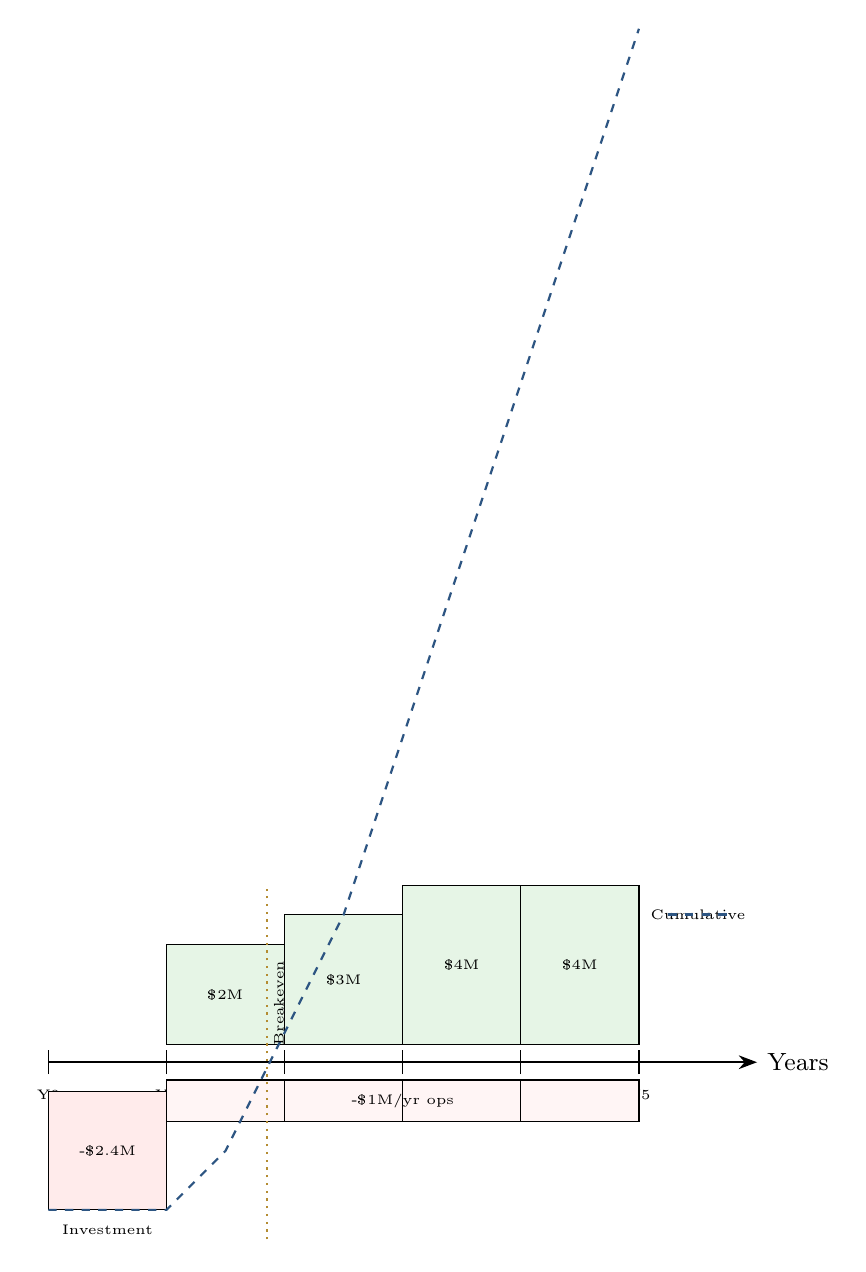
\begin{tikzpicture}[scale=0.75]
    % Investment timeline
    \draw[thick, -{Stealth}] (0, 0) -- (12, 0) node[right, font=\small] {Years};
    
    % Year markers
    \foreach \x/\yr in {0/Y0, 2/Y1, 4/Y2, 6/Y3, 8/Y4, 10/Y5} {
        \draw (\x, -0.2) -- (\x, 0.2);
        \node[below, font=\tiny] at (\x, -0.3) {\yr};
    }
    
    % Cost bars (negative)
    \draw[fill=costcolor] (0, -2.5) rectangle (2, -0.5);
    \node[font=\tiny] at (1, -1.5) {-\$2.4M};
    \node[font=\tiny, below] at (1, -2.6) {Investment};
    
    % Benefit bars (positive)
    \draw[fill=valuecolor] (2, 0.3) rectangle (4, 2);
    \node[font=\tiny] at (3, 1.15) {\$2M};
    
    \draw[fill=valuecolor] (4, 0.3) rectangle (6, 2.5);
    \node[font=\tiny] at (5, 1.4) {\$3M};
    
    \draw[fill=valuecolor] (6, 0.3) rectangle (8, 3);
    \node[font=\tiny] at (7, 1.65) {\$4M};
    
    \draw[fill=valuecolor] (8, 0.3) rectangle (10, 3);
    \node[font=\tiny] at (9, 1.65) {\$4M};
    
    % Ongoing costs
    \draw[fill=costcolor!50] (2, -1) rectangle (4, -0.3);
    \draw[fill=costcolor!50] (4, -1) rectangle (6, -0.3);
    \draw[fill=costcolor!50] (6, -1) rectangle (8, -0.3);
    \draw[fill=costcolor!50] (8, -1) rectangle (10, -0.3);
    \node[font=\tiny] at (6, -0.65) {-\$1M/yr ops};
    
    % Cumulative line
    \draw[thick, primary, dashed] (0, -2.5) -- (2, -2.5) -- (3, -1.5) -- (4, 0.5) -- (5, 2.5) -- (6, 5.5) -- (7, 8.5) -- (8, 11.5) -- (9, 14.5) -- (10, 17.5);
    
    % Breakeven point
    \draw[thick, dotted, accent] (3.7, -3) -- (3.7, 3);
    \node[font=\tiny, rotate=90] at (3.9, 1) {Breakeven};
    
    % Legend
    \node[font=\tiny] at (11, 2.5) {Cumulative};
    \draw[thick, primary, dashed] (10.5, 2.5) -- (11.5, 2.5);
    
\end{tikzpicture}
\caption{Investment Cash Flow Projection}
\end{figure}

\textbf{Description:} This chart shows the investment timeline with initial development cost of \$2.4M in Year 0, followed by annual net benefits (revenue minus operating costs) growing from \$2M to \$4M. The breakeven point occurs approximately 14 months after go-live. The dashed line shows cumulative value reaching \$17.5M over 5 years.

\subsection{Example 2: Strategic Alignment Map}

\begin{figure}[H]
\centering
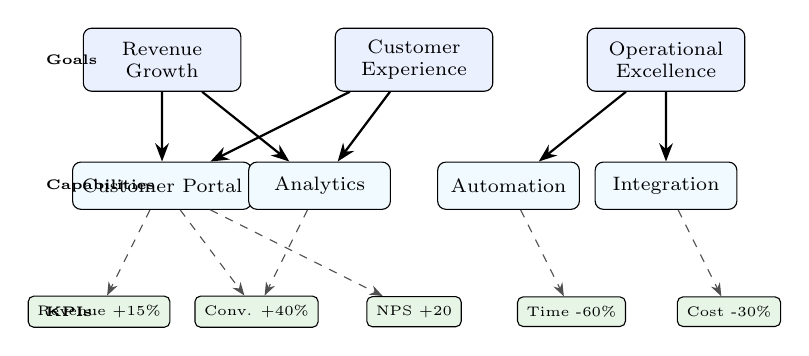
\begin{tikzpicture}[
    goal/.style={draw, fill=strategycolor, rounded corners=3pt, minimum width=2cm, minimum height=0.8cm, font=\scriptsize, align=center},
    capability/.style={draw, fill=kpicolor, rounded corners=3pt, minimum width=1.8cm, minimum height=0.6cm, font=\scriptsize},
    scale=0.8
]
    % Strategic Goals (top)
    \node[goal] (growth) at (-4, 4) {Revenue\\Growth};
    \node[goal] (cx) at (0, 4) {Customer\\Experience};
    \node[goal] (efficiency) at (4, 4) {Operational\\Excellence};
    
    % System capabilities (middle)
    \node[capability] (portal) at (-4, 2) {Customer Portal};
    \node[capability] (analytics) at (-1.5, 2) {Analytics};
    \node[capability] (automation) at (1.5, 2) {Automation};
    \node[capability] (integration) at (4, 2) {Integration};
    
    % KPIs (bottom)
    \node[draw, fill=valuecolor, rounded corners=2pt, font=\tiny] (rev) at (-5, 0) {Revenue +15\%};
    \node[draw, fill=valuecolor, rounded corners=2pt, font=\tiny] (conv) at (-2.5, 0) {Conv. +40\%};
    \node[draw, fill=valuecolor, rounded corners=2pt, font=\tiny] (nps) at (0, 0) {NPS +20};
    \node[draw, fill=valuecolor, rounded corners=2pt, font=\tiny] (time) at (2.5, 0) {Time -60\%};
    \node[draw, fill=valuecolor, rounded corners=2pt, font=\tiny] (cost) at (5, 0) {Cost -30\%};
    
    % Connections - goals to capabilities
    \draw[-{Stealth}, thick] (growth) -- (portal);
    \draw[-{Stealth}, thick] (growth) -- (analytics);
    \draw[-{Stealth}, thick] (cx) -- (portal);
    \draw[-{Stealth}, thick] (cx) -- (analytics);
    \draw[-{Stealth}, thick] (efficiency) -- (automation);
    \draw[-{Stealth}, thick] (efficiency) -- (integration);
    
    % Connections - capabilities to KPIs
    \draw[-{Stealth}, dashed, darkgray] (portal) -- (rev);
    \draw[-{Stealth}, dashed, darkgray] (portal) -- (conv);
    \draw[-{Stealth}, dashed, darkgray] (analytics) -- (conv);
    \draw[-{Stealth}, dashed, darkgray] (portal) -- (nps);
    \draw[-{Stealth}, dashed, darkgray] (automation) -- (time);
    \draw[-{Stealth}, dashed, darkgray] (integration) -- (cost);
    
    % Labels
    \node[font=\tiny\bfseries, anchor=west] at (-6, 4) {Goals};
    \node[font=\tiny\bfseries, anchor=west] at (-6, 2) {Capabilities};
    \node[font=\tiny\bfseries, anchor=west] at (-6, 0) {KPIs};
    
\end{tikzpicture}
\caption{Strategic Alignment Map}
\end{figure}

\textbf{Description:} This strategy map shows how system capabilities align with strategic goals and drive measurable KPIs. The Customer Portal supports both Revenue Growth and Customer Experience goals. Analytics enables data-driven improvements. Automation and Integration drive Operational Excellence. Each capability contributes to specific, measurable outcomes.

\subsection{Example 3: Portfolio Position}

\begin{table}[H]
\centering
\caption{System Portfolio Assessment}
\small
\begin{tabular}{@{}L{2.5cm}C{1.8cm}C{1.8cm}C{1.8cm}L{3.5cm}@{}}
\toprule
\textbf{System} & \textbf{Business Value} & \textbf{Technical Health} & \textbf{Strategy} & \textbf{Action} \\
\midrule
New Platform & \cellcolor{green!30}High & \cellcolor{green!30}High & Invest & Continue development \\
\addlinespace
Legacy CRM & \cellcolor{green!30}High & \cellcolor{red!30}Low & Migrate & Replace over 2 years \\
\addlinespace
Analytics Tool & \cellcolor{yellow!30}Medium & \cellcolor{green!30}High & Maintain & Optimize usage \\
\addlinespace
Old Reporting & \cellcolor{red!30}Low & \cellcolor{red!30}Low & Retire & Sunset in 6 months \\
\addlinespace
Mobile App & \cellcolor{green!30}High & \cellcolor{yellow!30}Medium & Evolve & Modernize UI \\
\bottomrule
\end{tabular}
\end{table}

% =============================================================================
% SECTION: NOTES
% =============================================================================
\section{Notes}

\subsection{Value Realization Management}

\begin{valuebox}[Value Realization Best Practices]
\begin{itemize}[nosep]
    \item \textbf{Define Clearly:} Specific, measurable benefit definitions
    \item \textbf{Assign Ownership:} Business owners accountable for realization
    \item \textbf{Track Continuously:} Regular measurement and reporting
    \item \textbf{Adjust Proactively:} Course-correct when off track
    \item \textbf{Learn Iteratively:} Refine estimates based on actuals
    \item \textbf{Communicate Results:} Share outcomes with stakeholders
    \item \textbf{Celebrate Success:} Recognize value delivery achievements
\end{itemize}
\end{valuebox}

\subsection{Governance Principles}

\begin{governbox}[Effective IT Governance]
\begin{itemize}[nosep]
    \item \textbf{Clear Ownership:} Every system has a business owner
    \item \textbf{Defined Decision Rights:} Who decides what is explicit
    \item \textbf{Appropriate Oversight:} Reviews proportional to risk
    \item \textbf{Transparency:} Open reporting on progress and issues
    \item \textbf{Accountability:} Consequences for commitments
    \item \textbf{Alignment:} Decisions support strategic objectives
    \item \textbf{Efficiency:} Governance enables rather than blocks
\end{itemize}
\end{governbox}

\subsection{Common Pitfalls}

\begin{warningbox}[Common Mistakes to Avoid]
\begin{enumerate}[nosep]
    \item \textbf{Unquantified Benefits:} Vague value without numbers
    \item \textbf{Hidden Costs:} Missing operational or integration costs
    \item \textbf{Optimistic Projections:} Unrealistic timelines or values
    \item \textbf{Missing Assumptions:} Undocumented dependencies
    \item \textbf{No Tracking:} Benefits claimed but never measured
    \item \textbf{Weak Governance:} Unclear ownership and decisions
    \item \textbf{Strategic Disconnect:} Investment without clear alignment
    \item \textbf{Ignoring TCO:} Focus on development, ignore operations
\end{enumerate}
\end{warningbox}

% =============================================================================
% SECTION: SOURCES
% =============================================================================
\section{Sources}

\subsection{Primary References}

\begin{enumerate}
    \item Clements, P., et al. (2010). \textit{Documenting Software Architectures: Views and Beyond} (2nd ed.). Addison-Wesley Professional.
    
    \item Kaplan, R., \& Norton, D. (1996). \textit{The Balanced Scorecard}. Harvard Business School Press.
    
    \item Ward, J., \& Daniel, E. (2012). \textit{Benefits Management: How to Increase the Business Value of Your IT Projects} (2nd ed.). Wiley.
    
    \item ISACA. (2012). \textit{COBIT 5: A Business Framework for the Governance and Management of Enterprise IT}.
    
    \item The Open Group. (2018). \textit{TOGAF Standard, Version 9.2}.
\end{enumerate}

\subsection{Supplementary References}

\begin{enumerate}[resume]
    \item Osterwalder, A., \& Pigneur, Y. (2010). \textit{Business Model Generation}. Wiley.
    
    \item Ross, J., Weill, P., \& Robertson, D. (2006). \textit{Enterprise Architecture as Strategy}. Harvard Business School Press.
    
    \item Brealey, R., Myers, S., \& Allen, F. (2020). \textit{Principles of Corporate Finance} (13th ed.). McGraw-Hill.
    
    \item PMI. (2017). \textit{The Standard for Portfolio Management} (4th ed.).
    
    \item ISACA. (2008). \textit{Val IT Framework 2.0}.
\end{enumerate}

\subsection{Online Resources}

\begin{itemize}
    \item Balanced Scorecard Institute: \url{https://balancedscorecard.org/}
    \item TOGAF: \url{https://www.opengroup.org/togaf}
    \item COBIT: \url{https://www.isaca.org/resources/cobit}
    \item Business Model Canvas: \url{https://www.strategyzer.com/}
\end{itemize}

% =============================================================================
% APPENDIX
% =============================================================================
\appendix

\section{Owner's View Checklist}

\begin{table}[H]
\centering
\small
\begin{tabular}{@{}L{10cm}C{2cm}@{}}
\toprule
\textbf{Item} & \textbf{Complete?} \\
\midrule
\multicolumn{2}{l}{\textbf{Business Case}} \\
\quad Benefits identified and quantified & $\square$ \\
\quad Costs estimated (development and operations) & $\square$ \\
\quad ROI/NPV/payback calculated & $\square$ \\
\quad Assumptions documented & $\square$ \\
\quad Sensitivity analysis performed & $\square$ \\
\midrule
\multicolumn{2}{l}{\textbf{Strategic Alignment}} \\
\quad Strategic goals identified & $\square$ \\
\quad Capability mapping completed & $\square$ \\
\quad Alignment validated with stakeholders & $\square$ \\
\quad Portfolio context documented & $\square$ \\
\midrule
\multicolumn{2}{l}{\textbf{Governance}} \\
\quad Sponsorship established & $\square$ \\
\quad Business owner assigned & $\square$ \\
\quad Decision rights defined & $\square$ \\
\quad Oversight mechanisms in place & $\square$ \\
\midrule
\multicolumn{2}{l}{\textbf{Metrics and Tracking}} \\
\quad KPIs defined with targets & $\square$ \\
\quad Data sources identified & $\square$ \\
\quad Reporting mechanism established & $\square$ \\
\quad Benefit tracking planned & $\square$ \\
\midrule
\multicolumn{2}{l}{\textbf{Risk Management}} \\
\quad Business risks identified & $\square$ \\
\quad Impact quantified & $\square$ \\
\quad Mitigations defined & $\square$ \\
\quad Risk owners assigned & $\square$ \\
\bottomrule
\end{tabular}
\end{table}

\section{Glossary}

\begin{description}[style=nextline, leftmargin=3cm, labelwidth=2.8cm]
    \item[Benefit] A positive business outcome delivered by the system.
    
    \item[Business Case] Justification for investment based on costs and benefits.
    
    \item[Capability] A business ability enabled by the system.
    
    \item[Cost of Ownership] Total lifecycle cost including development and operations.
    
    \item[Governance] Framework of decision rights and accountability.
    
    \item[IRR] Internal Rate of Return; discount rate where NPV equals zero.
    
    \item[KPI] Key Performance Indicator measuring business outcomes.
    
    \item[NPV] Net Present Value; sum of discounted future cash flows.
    
    \item[Payback Period] Time required to recover initial investment.
    
    \item[Portfolio] Collection of systems managed as a group.
    
    \item[ROI] Return on Investment; ratio of net benefit to cost.
    
    \item[Sponsor] Executive who authorizes and funds the system.
    
    \item[Strategic Alignment] Connection between system and business strategy.
    
    \item[TCO] Total Cost of Ownership over system lifecycle.
    
    \item[Value Stream] Sequence of activities delivering value to customers.
\end{description}

% =============================================================================
% END DOCUMENT
% =============================================================================

\end{document}
